\section{Business Model}
\begin{figure}[H]
\centering
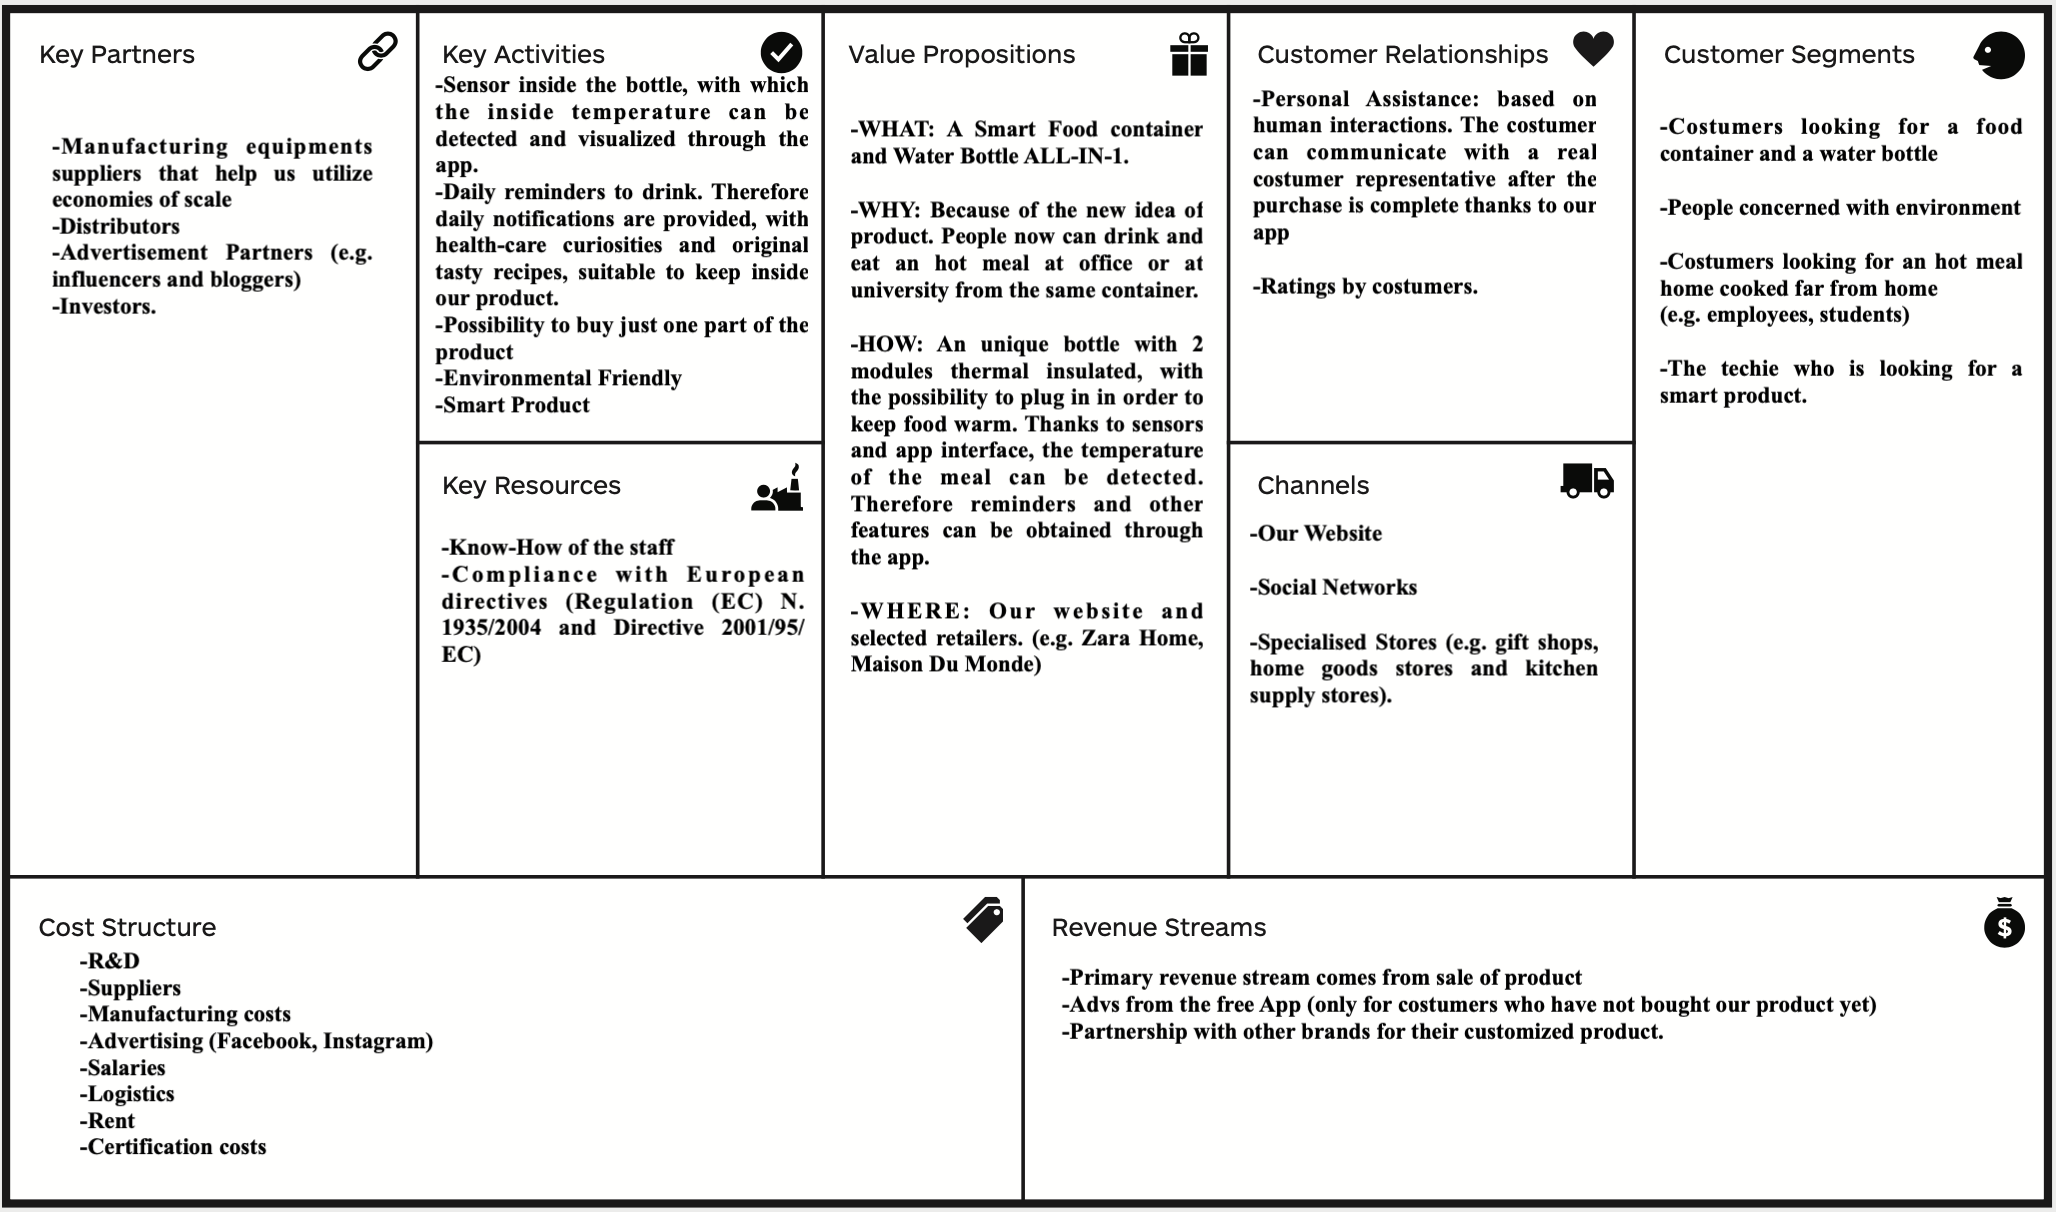
\includegraphics[width=1\textwidth]{images/BMC.png}
\caption{BottAll Business Model Canvas}
\end{figure}
The above diagram exhibits our key activities which will convince our potential costumer to choose BottlAll. We offer a smart product, with a temperature sensor. Furthermore we offer the possibility to visualize the temperature directly in our BottApp. In addition, daily reminders to drink are provided. Then, daily notifications with health-care curiosities, and original tasty recipes suitable for our product will be displayed in the App. Last but not least, we are environmental friendly. Thanks to BottAll, our costumer refuses to contribute buying more plastic bottles or plastic food containers which contributes to pollute our world.\\
As shown above, our business will outsource manufactured steel containers and all manufacturing items which will be assembled in our factory. Therefore, thanks to the support of our suppliers, we aim to produce economy of scale in order to reduce the production costs and rising the sales volumes. Our product will be compliant with European directive n. 1935/2004 (CE) and directive 2001/95/EC (i.e. materials in contact with food).\\
Selling channels will be primarily our website, then social networks and selected retailers, such as Zara Home and Maison Du Monde.\\
Finally, our mainly revenue streams will come from sales of product. They will also arise from advertisements or the free App, which will be present only for customers who have not bought our product yet. Then, we are intended to arrange strategic partnerships with other brands for their customized product. 